\documentclass[oldfontcommands,oneside,a4paper,11pt]{article} 
\usepackage{fontspec}
\usepackage{natbib}
\usepackage{booktabs}
\usepackage{xltxtra} 
\usepackage{polyglossia} 
\setdefaultlanguage{french} 
\usepackage[table]{xcolor}
\usepackage{multirow}
\usepackage{gb4e} 
\usepackage{graphicx}
\usepackage{float}
\usepackage{lscape}
\usepackage{hyperref} 
\hypersetup{bookmarks=false,bookmarksnumbered,bookmarksopenlevel=5,bookmarksdepth=5,xetex,colorlinks=true,linkcolor=blue,citecolor=blue}
\usepackage[all]{hypcap}
\usepackage{memhfixc}

\bibpunct[~: ]{(}{)}{,}{a}{}{,} 


\setmainfont[Mapping=tex-text,Numbers=OldStyle,Ligatures=Common]{Charis SIL} %ici on définit la police par défaut du texte


\newfontfamily\phon[Mapping=tex-text,Ligatures=Common,Scale=MatchLowercase,FakeSlant=0.3]{Charis SIL}  
\newcommand{\ipa}[1]{{\phon #1}} %API tjs en italique
\newcommand{\ipac}[1]{{\tiny #1}} 
\newfontfamily\cn[Mapping=tex-text,Ligatures=Common,Scale=MatchUppercase]{MingLiU}%pour le chinois
\newcommand{\zh}[1]{{\cn #1}}
\newcommand{\petit}[1]{\tiny#1}
\newcommand{\sig}{\begin{math}\Sigma\end{math}} 
\newcommand{\ra}{$\Sigma_1$} 
\newcommand{\rc}{$\Sigma_3$} 
\newcommand{\grise}[1]{\cellcolor{lightgray}\textbf{#1}}


\begin{document}
%\OnehalfSpacing
\title{Projet de recherche} 
\author{Guillaume Jacques}
\maketitle

\sloppy
\tableofcontents

\section{Animation de la recherche et enseignement}

\subsection{Enseignement et direction de travaux}
Suite à l'obtention de mon habilitation à diriger des recherches, j'envisage de consacrer un temps plus important à la supervision d'étudiants en mastaire et en thèse. Je compte diriger suffisamment de thèses pour couvrir l'ensemble des langues (et dialectes) rgyalronguiques et kiranti qui restent à décrire, ainsi que pour approfondir des points spécifiques sur les langues les mieux dotées. Mis à part les langues de tradition orale, j'ai également l'intention de former des étudiants en tangoute, qui pourront prolonger mes travaux et valoriser le corpus que j'ai déjà transcrit dans cette langue -- outre des thèses en linguistique, je pourrai diriger des recherches sur l'histoire ou le bouddhisme tangoute.
 
Je m'investirai davantage dans l'enseignement et l'organisation du mastaire conjoint Inalco-Paris III afin de découvrir, former et soutenir les étudiants prometteurs et en particulier les aider à acquérir rapidement la capacité à rédiger des travaux publiables. Les enseignements que je donnerai, outre ceux de morphosyntaxe générale que je propose actuellement, comprendront la linguistique historique et des formations (concentrées sur une semaine) à des outils informatiques.

J'espère  fonder une école de linguistique sino-tibétaine, dont chaque membre devra se charger de la documentation complète (avec corpus d'enregistrements d'au moins une dizaine d'heures, dictionnaire et grammaire) d'une langue rgyalronguique, tibétaine ou  kiranti, mais aussi se former en informatique (Perl/Python, transducteurs, langages formels, \LaTeX, R)  et en linguistique historique (indo-européenne et sino-tibétaine). En particulier, les étudiants chinois de linguistique en France forment un vivier idéal, car il connaissent déjà la langue de contact et on une plus grande facilité d'accès au terrain.

Ces trois domaines sont traditionnellement séparés, mais je suis convaincu qu'ils sont complémentaires, et que le domaine gagnerait considérablement en rigueur et en fiabilité empirique et théorique si non pas quelques individus isolés, mais toute une génération de linguistes, pouvaient combiner ces compétences.

%La linguistique de terrain permet d'effectuer un travail de description utile à long terme, aide à acquérir la connaissance pratique d'une langue peu connue et rend possible la découverte de phénomènes complètement inconnus.  La linguistique informatique est utile pour traiter plus efficacement le corpus transcrit, et automatiser les tâches qui peuvent l'être. D'autre part, la connaissance de la théorie des langages formels et automates permet une approche théorique implémentable  aussi bien en phonologie qu'en morphologie ou qu'en syntaxe. La linguistique historique, enfin, apporte une dimension explicative qui enrichit l'approche   synchronique et formelle des données.

Outre les langues sino-tibétaines, je développerai aussi des études sur les langues d'Amérique du nord (en particulier sioux et algonquien) qui sont encore sous-représentées chez les linguistes français. Même si je n'ai pas fait de terrain sur ces langues, j'ai lu des textes en ojibwe et en lakhota (avec traduction non interlinéaire), et j'ai écrit quelques articles sur l'algonquien (\citealt{jacques12bear, jacques13arapaho, jacques15directionality}); je pense avoir acquis assez de connaissances sur les familles algonquiennes et sioux, aussi bien en linguistique historique qu'en morphosyntaxe, pour guider les étudiants vers des travaux publiables dans de bonnes revues. Je pourrai ainsi contribuer à combler une lacune dans les recherches typologiques et descriptives menées aujourd'hui en France.

\subsection{Projets de recherche}
Je compte d'une part m'investir dans le Labex \textit{Empirical Foundations of Linguistics} (EFL), et d'autre part continuer à monter des projets ANR. Ces activités me permettront de formaliser mes collaborations scientifiques avec des membres d'autres équipes de recherches, d'avoir des ressources pour engager des informaticiens afin de développer des outils (voir section \ref{sec:outils}) et des bases de données, et aussi pour pouvoir financer les thèses et les missions de terrain des étudiants.

Je compte commencer à rédiger un projet ANR en collaboration avec Benoît Sagot (INRIA) sur les méthodes formelles en linguistique historique (voir section \ref{sec:formelles}) dès la fin du projet ANR HimalCo dont je suis le porteur actuellement, c'est à dire fin 2015 ou mi-2016 si nous parvenons à obtenir une prolongation de six mois.

\subsection{Organisation de conférences et de rencontres de chercheurs}
%Si je n'ai jamais pour le moment organisé de grande conférence internationale, j'envisage de me charger de ce type de tâches dans la suite de ma carrière.

Dans les années qui vont suivre, je compte organiser des journées d'étude sur des sujets ciblés. En particulier, j'ai l'intention d'organiser des colloques sur les langues kiranti et les langues rgyalronguiques ainsi que sur les études tangoutes. Ces rencontres pourront avoir lieu en France mais aussi en Chine ou au Népal, afin de permettre aux locuteurs des langues concernées de participer plus facilement. 

%Ensuite, je participerai à la mise en place de conférences de typologie généralistes de plus grande envergure à Paris (comme \textit{Syntax of the World's languages}).



\subsection{Activités éditoriales}
Je continuerai dans les années qui vont suivre mon travail de rédacteur en chef de la revue \textit{Cahiers de linguistique d'Asie orientale}, mais je compte m'investir dans d'autres revues. En particulier, à partir de mi-2015, je serai responsable (pour au moins 4 ans) de la linguistique historique en collaboration avec Michael Weiss (\textit{area editor for Historical Linguistics}) dans la nouvelle revue \textit{Linguistic Vanguard} (Mouton de Gruyter). 

En tant que responsable de revues, ma vision est de privilégier les articles présentant des données fiables,  revérifiables et originales, et de promouvoir l'inclusion de suppléments (en particulier les fichiers sons, mais aussi d'autres données phonétiques) dans la version en ligne des articles. D'une façon générale je souhaite contribuer à élever le standard général des exigences sur la qualité des données dans les articles de linguistique. % et aussi bien en tant que relecteur qu'éditeur, j'incite les auteurs à limiter au maximum les phrases isolées sorties de leur contexte.

\section{Recherche}

\subsection{Grammaire et corpus de référence du japhug}
Ma priorité à moyen terme est de finir une grammaire de référence du japhug, accompagnée d'un dictionnaire et d'un corpus de textes disponibles en ligne. Une première version du dictionnaire sera disponible en ligne d'ici mi-2015, et le corpus sera progressivement publié sur le site Pangloss. 

Ce corpus, qui dépasse 60h de textes enregistrés (sans compter les phrases isolées et les listes de mots), aura besoin d'être complété toutefois par davantage de conversations -- il n'en comprend actuellement seulement qu'une heure. Or, les conversations, par opposition aux histoires et aux textes procéduraux, sont indispensables pour éclaircir de nombreux aspects de la grammaire, en particulier le TAM et l'usage des particules de fin de phrase. En outre, pour les textes procéduraux, je compte collecter davantage de données vidéo. 

Néanmoins, je considère déjà disposer d'un corpus relativement représentatif pour une description de la langue assez détaillée. C'est donc la rédaction de la grammaire qui est maintenant pour moi la tâche prioritaire.



Si j'ai déjà publié une grammaire en chinois (\citealt{jacques08zh}), celle-ci, du fait des contraintes de la collection où elle a été publiée, est relativement courte (472 pp -- j'avais dû raccourcir le manuscrit) et n'est pas utilisable par les typologues occidentaux à cause de la barrière de la langue. Par ailleurs, ma connaissance du japhug est considérablement plus avancée maintenant qu'en 2006-2007 (lorsque je rédigeais ce livre), et mon corpus actuel est six fois plus long qu'à cette époque. Il est donc indispensable d'écrire une nouvelle grammaire en anglais, destinée aux typologues et aux comparatistes.  Ce travail n'est pas redondant avec la grammaire de 2008, car il s'adresse à une audience différente, et sera fondé sur un corpus d'une taille beaucoup plus conséquente.

Depuis 2010, j'ai publié une série d'articles en anglais sur plusieurs points de la morphosyntaxe du japhug, qui peuvent être remaniés comme chapitres de grammaire en ajoutant de nouveaux exemples, en supprimant les redondances et en les intégrant à l'ensemble du manuscrit. Si l'on prend en compte d'autres sections déjà partiellement rédigées, je dispose déjà en tout de 290 pages en anglais, mais ces matériaux n'ont pas encore été combinés en un  tout cohérent.

  J'ai soumis cinq articles qui pourront être intégrés sous forme remaniée à la grammaire sur la phonologie (\textit{illustration of the IPA}), les comparatives, le générique, les constructions causatives et les relatives. Je compte soumettre en 2015 et 2016 au moins cinq articles sur la morphosyntaxe du japhug: les numéraux et les classificateurs (pour un Festschrift), le préfixe spontané / autobénéfactif, le discours indirect hybride, les complétives et l'évidentialité. 
  
  Lorsque tous ces articles seront achevés, je me consacrerai pleinement  à synthétiser toutes les sections déjà rédigées et à les compléter, ainsi qu'à écrire les sections qui peuvent difficilement mener à un article (dans les domaines de la grammaire où le japhug n'est pas typologiquement inhabituel).

J'estime à quatre ans, à raison de 150 pages par an (ajoutées à celles déjà écrites), le délai nécessaire minimal pour compléter la première version complète de la grammaire (pour 2018-2019).

\subsection{Grammaire comparée des langues rgyalronguiques et des langues kiranti}
La grammaire du japhug sera la première pierre d'un édifice plus général -- la grammaire comparée (synchronique et diachronique) des langues rgyalronguiques et kiranti, les deux branches de la famille sino-tibétaine dont la morphologie verbale est la plus complexe (voir les cartes  \ref{fig:rgy}  et \ref{fig:kirant}). Ces deux branches comprennent respectivement 10 et 22 langues au minimum -- soit une quantité de données plus grande que l'ensemble de la famille algonquienne, et il me semble préférable de concentrer mes efforts sur ces deux groupes plutôt que d'essayer de maîtriser l'ensemble des données sino-tibétaines.

   \begin{figure}[h]
   \caption{Langues rgyalronguiques (en grisé; Sichuan tibétain, Chine) }  \label{fig:rgy}  \centering
 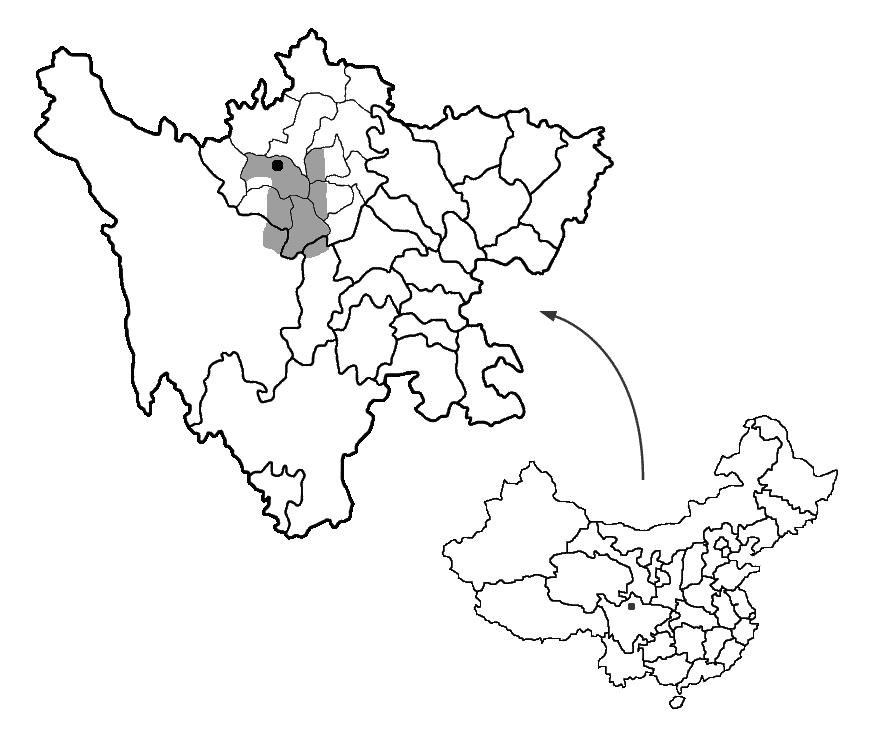
\includegraphics[width=0.6\textwidth]{carte.JPG}
 \end{figure}
Ce projet de recherche sera nécessairement collectif, car la masse des données à traiter rend impraticable une approche isolée. Il comprendra quatre parties: descriptions des langues et collecte de données, phonologie comparée du rgyalronguique, phonologie historique du khaling et enfin morphosyntaxe comparée.

 \begin{figure}[h]
   \caption{Langues kiranti (est du Népal)} \label{fig:kirant}   \centering
  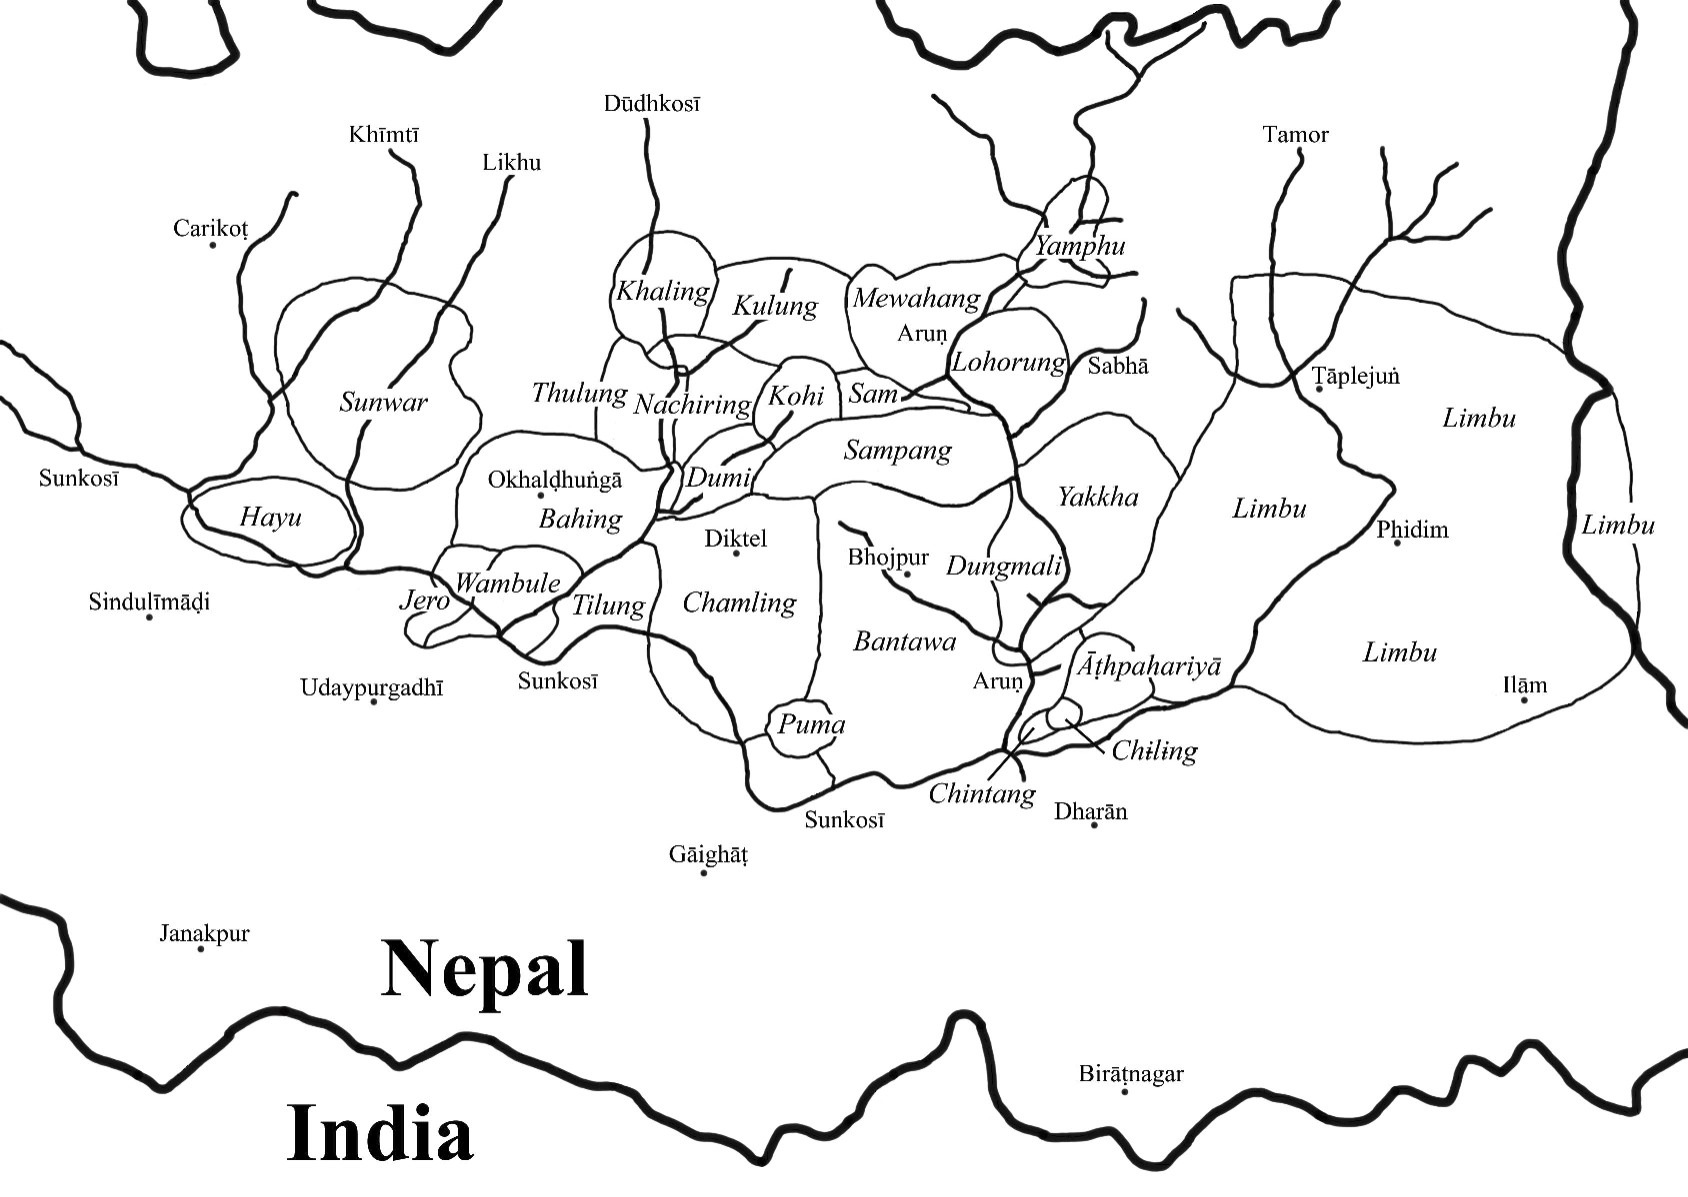
\includegraphics[width=\textwidth]{Kirant.jpeg} 
 \end{figure}
 
\subsubsection{Collecte de données}
Une recherche comparative requiert des données riches, fiables et complètes sur toutes les langues étudiées, et à ce titre cette entreprise n'est pas réalisable sur la base exclusive de la grammaire japhug.

Je ne compte pas d'ici 2020 me charger de rédiger de grammaire autre que celle du japhug. Néanmoins, je continuerai à travailler sur trois autres langues, le khaling (kiranti), le stau et le situ (rgyalronguique), collecterai des enregistrements, et écrirai des articles sur des points spécifiques de morphosyntaxe, probablement en collaboration (avec Aimée Lahaussois, Anton Antonov, Lai Yunfan et Gong Xun). Il est probable que certains de ces articles pourront mener à des contributions théoriques plus générales et conduire notre recherche en typologie dans des directions nouvelles (voir section \ref{sec:morphosyntaxe}).


\subsubsection{Phonologie et morphologie comparée du rgyalronguique} \label{sec:comparee.rgy}
Dans mes travaux précédents, en particulier \citet{jacques04these} et \citet{jacques14esquisse}, j'ai présenté une reconstruction préliminaire du proto-rgyalrong, et ai établi un certain nombre de lois phonétiques. Toutefois, ces résultats, basés sur des données incomplètes, devront être intégralement revus lorsque, dans cinq à dix ans, on disposera de lexiques fiables sur toutes les langues rgyalronguiques.

Le lexique comparatif des langues rgyalronguiques comprend actuellement plus de 700 groupes de cognats. Etant donné la proximité de ces langues, il sera sans doute possible de doubler le nombre de cognats avec des lexiques plus complets,  d'affiner les lois déjà connues et d'en découvrir de nouvelles. 

Outre la reconstruction phonologique proprement dite, il est nécessaire d'intégrer la morphologie dans ces reconstructions, en particulier les alternances de thèmes verbaux réguliers et irréguliers et les dérivations verbales et dénominales. Si certaines alternances vocaliques peuvent être expliquées comme résultant de la fusion du radical verbal avec des suffixes (\citealt[357-8]{jacques04these}) ce n'est pas le cas de la majorité d'entre elles en particulier en zbu (\citealt{jackson04showu}), et leur origine reste jusqu'à ce jour un mystère.

\subsubsection{Phonologie et morphologie historique du khaling}
En kiranti, je compte au moins dans un premier temps me focaliser sur la comparaison du khaling et du dumi (\citealt{driem93dumi}) et du koyi (\citealt{lahaussois09}), car ces trois langues forment un sous-groupe clair au sein du kiranti et leur systèmes verbaux sont facilement comparables -- ce qui n'est pas le cas avec des langues kiranti plus éloignées comme le thulung ou le limbu.

Ce groupe présente une situation presque idéale pour le comparatiste. En effet, le khaling est très conservateur du point de vue des attaques (en particulier les groupes de consonnes initiaux) mais très innovateur en ce qui concerne les voyelles et les consonnes finales, alors qu'à l'inverse, le dumi a perdu les groupes de consonnes initiaux, mais préserve bien en revanche les consonnes finales. 


J'ai déjà étudié la tonogénèse en khaling, dans un article soumis à un volume collectif sur les alternances tonales dans les paradigmes verbaux (en cours d'évaluation). J'y montre que les tons du khaling ont deux origines: la simplification des consonnes finales et la réduction de dissyllabes (qui sont préservées en dumi). La linguistique historique permet en outre de rendre compte des alternances observées en synchronie.

Je compte par la suite préparer un lexique comparatif des verbes khaling et dumi, ainsi qu'une reconstruction détaillée du système verbal de leur ancêtre commun, en combinant méthode comparative et reconstruction interne.

\subsubsection{Morphosyntaxe comparée}
La grammaire comparée ne se limite pas à une liste de morphèmes reconstruits. Une fois les lois phonétiques établies, il devient possible d'effectuer une comparaison détaillée de l'ensemble des constructions grammaticales dans les langues étudiées.

Il est difficile, à ce stade de nos connaissances des langues rgyalronguiques autres que le japhug, de prévoir quels seront les sujets d'étude les plus prometteurs dans ce domaine. Je compte au moins étudier en détail les deux questions suivantes:
\begin{enumerate}
\item L'histoire des systèmes d'indexation de personne en rgyalronguique et en kiranti: Dans quelle mesure les ressemblances entre ces deux groupes peuvent-elles s'expliquer par une évolution parallèle ou par un héritage commun (\citealt{jacques12agreement}) et quel système d'indexation est-il possible de reconstruire pour leur ancêtre commun?
\item Les préfixes de nominalisation (qui sont cognats entre rgyalronguique et kiranti) et leurs différentes fonctions syntaxiques (dans les relatives, les complétives et les subordonnées de manière).
\end{enumerate}

 



\subsection{Typologie des changements phonétiques } \label{sec:phonetique}
De tous les domaines de la linguistique historique, c'est sans doute la phonologie dans laquelle la formulation de lois générales est le moins problématique. 

A court et moyen terme, je compte essentiellement écrire des articles sur des points spécifiques, comme les origines diachroniques de certains sons rares ou de changements peu habituels, dans la lignée des mes articles \citet{jacques11lingua} (sur les fricatives aspirées), \citet{michaud-jacques12nasalite} (sur la nasalité) et \citet{jacques13arapaho} (sur la phonologie historique de l'arapaho). 

En particulier, je compte effectuer une recherche sur le passage des occlusives labiales en vélaires \ipa{*p} $\rightarrow$ \ipa{k}  comme en arapaho (\citealt{goddard74arapaho}) et en strait salish (où elles finissent comme des affriquées palatales, voir \citealt[10-11]{kuipers02salish}). Ce travail traitera en particulier des changements en chaîne auxquels \ipa{*p} $\rightarrow$ \ipa{k}  participe dans les langues où il est attesté.

Je m'intéresse aussi à la question de la débuccalisation des consonnes (soit leur disparition, soit leur passage à des glottales \ipa{h} ou \ipa{ʔ}). Parmi tous les types de changements, c'est probablement ceux dont le caractère unidirectionnel est le plus clair. Néanmoins, la disparition des consonnes peut suivre de nombreux chemins distincts, dont toutes les étapes ne sont pas nécessairement unidirectionnelles. Cette question mérite d'être traitée en tenant compte à la fois du contexte où le changement a lieu mais aussi de la structure générale du système (en particulier les débuccalisations sont souvent attestées comme premier membre d'un changement en chaine). Parmi les langues que j'étudie, le groupe kiranti offre des cas particulièrement intéressants et mal compris de débuccalisation des occlusives initiales (en yamphu, yakkha et belhare), qui méritent d'être présentés à un public plus large de phonologues et de diachroniciens.


A plus long terme, la compilation d'une base de données sur les changements phonétiques, basée sur des sources primaires mais également sur des synthèses telles que  \citet{kuemmel07wandel} ou \citet{blevins04evolutionary, blevins08naturalness} est réalisable en équipe (avec des collègues tels qu'Alexis Michaud).

 

\subsection{Morphosyntaxe panchronique} \label{sec:morphosyntaxe}
Dans le domaine de la morphosyntaxe, je m'intéresse d'une part aux systèmes d'indexation et de voix et d'autre part à la typologie de l'ordre des mots, car c'est sur ces sujets que les données du japhug m'ont permis d'écrire les articles dont je suis le plus satisfait (en particulier \citealt{jacques12incorp}, \citealt{jacques13harmonization}, \citealt{jacques14antipassive}).

Je n'exclus pas de travailler sur d'autres aspects de la morphosyntaxe dans une perspective typologique, en fonction des phénomènes que je découvrirai  dans les langues rgyalronguiques et kiranti dans mes recherches futures.

\subsubsection{Évolution des systèmes d'indexation} \label{sec:indexation}
 Mes travaux sur la morphologie comparée des langues rgyalronguiques et kiranti pourront être intégrés dans un cadre plus large, celui des principes généraux des changements diachroniques dans les systèmes verbaux à indexation polypersonnelle.  
 
 Ce programme de recherche, non limité au sino-tibétain, intégrera des données d'autres familles à indexation complexe, notamment celles de familles d'Amérique du nord comme l'algonquien, le sahaptien et le sioux. 

Une première étape de ce travail est \citet{jacques15directionality}, dans lequel nous avons découvert certaines récurrences dans le fonctionnement des changements analogiques dans les langues algonquiennes, en particulier dans la réfection du \textit{conjunct order}. Ce travail amène à la constatation suivante:  \textbf{les formes les plus courantes sont celles qui résistent le mieux à l'analogie, et sur la base desquelles les généralisations analogiques opèrent}. Ainsi, les formes du singulier résistent mieux à l'analogie que les formes du pluriel, la troisième personne que la première ou la seconde, les formes directes que les formes inverses ou `locales'.

Je souhaiterais tester la validité de cette idée, et la quantifier par des études de corpus sur des langues de familles différentes. Dans un article soumis à une revue, je montre un contre-exemple apparent dans les langues sioux à l'idée que la troisième personne est toujours la forme pivot sur laquelle se fondent les analogies: dans le cas de verbes où la première personne est la plus fréquente (les verbes de cognition comme `penser' ou `savoir'), il peut arriver que l'analogie parte de la première personne, et que la troisième personne soit refaite.
 
 Une autre question importante est la genèse des morphèmes portemanteaux  (notamment pour les marques `locales' $1\rightarrow2$ et $2\rightarrow1$, voir \citealt{heath98skewing}). J'ai déjà contribué à cette question dans le cas du rgyalronguique (\citealt{jacques15generic}), et compte l'aborder dans les langues algonquiennes et sioux, dont la phonologie historique est suffisamment bien élucidée pour pouvoir entreprendre ce type de recherches. 
 
 
 \subsubsection{Origine diachronique des marques de voix} 
Dans  la continuation de mon article \citet{jacques14antipassive}, j'envisage d'écrire une monographie sur l'origine diachronique des marques de voix dans les langues du monde, dans laquelle j'inclurai les marques de personne indéfinie / générique et l'incorporation.

C'est un sujet sur lequel une vaste littérature  existe depuis une trentaine d'années, mais la quasi-totalité des travaux sur la grammaticalisation négligent les lois phonétiques et la méthode comparative, surtout dans le cas de langues non-indo-européennes (voir la critique de \citealt{heath98hermit}).

On dispose de travaux réutilisables par les non-spécialistes sur la diachronie de nombreuses familles de langues non-européennes qui sont encore sous-employés dans les approches plus générales (en particulier dans le cas de l'algonquien, du sioux et du salish, et bien sûr aussi à terme du rgyalronguique et du kiranti). Une synthèse de ces recherches est donc réalisable.

 Comme \citet{haspelmath90passive}, la question qui m'intéresse le plus est celle de l'unidirectionnalité des changements diachroniques. Il est manifeste que des exceptions à certains changements supposés unidirectionnels ont été mises au jour (\citealt{norde09degrammaticalization}), et  l'on ne peut nier que certains changements sont bidirectionnels. Néanmoins, il est tout aussi clair que les changements unidirectionels existent, et les identifier et en compiler la liste est une priorité pour établir une théorie générale des évolutions linguistiques.  
 
% Il est aussi crucial de porter aux étapes intermédiaires entre les constructions source et arrivée. Il y a par exemple de multiples chemins qui mènent d'un verbe à une marque de voix:
 
 
  \subsubsection{Typologie des langues OV préfixantes} 
 Il existe peu de langues strictement verbe final qui soient majoritairement préfixantes -- seules les langues athabasques, sioux, rgyalronguiques, et à moindre mesure le caucasique du nord-ouest et le ket combinent ces deux propriétés. Dans l'article  \citet{jacques13harmonization}, j'ai proposé que la rareté des langues de ce type ne résulte pas de l'effet d'une contrainte psycholinguistique, mais d'une contingence historique (la propagation du type SOV suffixant en Eurasie par remplacement et / ou contact de langue).  En effet, aussi bien le rgyalronguique que l'athabasque présentent des cas clairs de grammaticalisation de verbes comme préfixes alors que des suffixes auraient été attendus à partir de la structure synthétique correspondante.
 
Pour approfondir cette question, je compte étudier les propriétés morphosyntaxiques que ces langues ont en commun en plus de l'ordre des mots et des affixes en comparaison avec les langues SOV suffixantes (le type dravidien-altaïque-andéan) -- par exemple, le fait que ces langues semblent toutes privilégier les relatives à tête interne, le rapport assez élevé de formes verbales finies par rapport aux formes non-finies dans les corpus de textes etc. 

Comme cette question ne concerne qu'un nombre limité de famille de langues, un tel projet est tout à fait réalisable, et pourra mener à des progrès importants pour affiner notre connaissance des universaux morphosyntaxiques.

\subsubsection{Evidentialité nominale}
Suite à l'article \citet{jacques14auditory} sur le démonstratif auditif en khaling, Alexandra Aikhenvald m'a demandé d'écrire une entrée sur l'évidentialité non propositionnelle (marquée dans les groupes nominaux, notamment par des démonstratifs) pour le \textit{Oxford Handbook of Evidentiality}. Je rédigerai cette contribution en 2015, pour parution potentielle en 2016.

Il est possible que je continue par la suite à travailler sur ce sujet, en fonction de ce que je découvrirai en préparant l'article pour l'encyclopédie. En particulier, il pourrait être intéressant d'inclure dans une telle étude non seulement les systèmes démonstratifs, mais aussi les langues omniprédicatives ayant des marques d'évidentialités pouvant apparaître aussi bien sur les verbes que sur les noms.


%Un problème majeur en linguistique historique est l'apparente imprédictibilité des changements sémantiques. Le seul outil dont disposent actuellement les linguistes pour juger de la plausibilité d'une comparaison particulière (lorsqu'elle est phonétiquement possible) est la recherche d'exemples de changements sémantiques du même type attestés dans d'autres langues.
%
%Comme la méthode comparative n'offre aucune méthode pour reconstruire la sémantique, on en est réduit à chercher des exemples dans les langues pour lesquelles on dispose de données anciennes -- soit une infime minorité, et presque exclusivement dans quelques familles d'Eurasie. Baser un modèle de changement sémantique sur un corpus aussi restreint réduit sa représentativité, surtout si l'on souhaite pour l'appliquer à des langues d'autres continents, notamment celles parlées traditionnellement par des chasseurs-cueilleurs.
% 
%\citet{urban11semantic} propose une procédure pour enrichir la liste connue des changements sémantiques et déterminer leur directionnalité, même sur des langues sans textes anciens. Il propose que les extensions sémantiques que l'on peut détecter sur la base de données synchroniques, notamment dans les mots composés (par exemple, le fait que de nombreuses langues ont un mot composé comprenant la racine de `peau' dans le mot pour `écorce', mais jamais l'inverse) suivent les même règles et ont la même directionnalité que les changements sémantiques diachroniques. (le changement `peau' $\rightarrow$ `écorce' est unidirectionnel). Pour tester cette hypothèse, il confronte une base de donnée sur les extensions sémantiques dans un échantillon de 149 langues de familles diverses, qu'il compare ensuite à des changements historiques attestés.
%
%Cette procédure mériterait d'être appliquée plus systématiquement, voire automatisée dans la mesure du possible. L'article en question n'aborde qu'une courte liste de noms du `vocabulaire de base', et il n'est pas sûr que cette méthode soit aussi facile à utiliser pour les verbes, car les composés verbaux -- les verbes à incorporation -- n'existent pas dans toutes les langues, et les évolutions sémantiques avec les affixes directionnels/locatifs (comme les préverbes dans les langues indo-européennes) ne suit pas nécessaire le même type de chemins.

\subsection{Méthodes formelles en linguistique historique} \label{sec:formelles}

En linguistique historique, le problème fondamental encore non résolu n'est pas la formulation d'hypothèses possibles, mais plutôt la comparaison entre hypothèses basées sur le même ensemble de données. 

A l'heure actuelle, il est possible de déterminer si (1) une hypothèse est cohérente (2) s'il existe des données qui l'infirment et (3) si les changements historiques postulés ont des parallèles typologiques. 

Dans les cas où plusieurs hypothèses concurrentes satisfont les trois conditions ci-dessus, les seules méthodes automatiques d'évaluation qui existent en linguistique historique portent sur la phylogénie, où les méthodes phylogénétiques développées en biologie ont été appliquées (suite à l'article de \citealt{gray03ie}). En reconstruction de la phonologie et de la morphologie, en revanche, aucun outil n'existe autre que l'intuition des chercheurs. 

Le concept de la \textit{longueur de description minimale} (LDM) développé en théorie de l'information (\citealt{rissanen84}) a déjà été appliqué à la comparaison de modèles alternatifs en morphologie (\citealt{walther14compactness}). C'est un moyen pour mesurer la complexité relative d'hypothèses concurrentes ayant la même puissance prédictive. 

Certains auteurs ont déjà proposé d'utiliser la  LDM en linguistique historique (par exemple, \citealt{hiltunen12mdl}), mais leur perspective (l'alignement automatique des mots à partir de données brutes) est tout à fait différente, et assez éloignée des besoins réels des linguistes diachroniciens.

Même si l'étude des changements phonétiques réguliers est le domaine de la linguistique historique le plus facile à formaliser, l'application de la LDM à des transducteurs modélisant les changements phonétiques n'est pas triviale, et un tel projet requiert une collaboration étroite entre diachroniciens et informaticiens. C'est en particulier avec Benoît Sagot (co-auteur de \citealt{walther14compactness}) et Johann-Mattis List (qui effectuera un post-doc au CRLAO en 2015) que je compte mener à bien cette entreprise, dans le cadre du Labex \textit{Empirical foundations of linguistics} et peut-être d'un futur projet ANR.



 
%
%\subsection{Changements phonétiques}
%Il est possible, en utilisant soit des langages de script (Perl ou Python), soit des transducteurs (XFST), de concevoir des programmes appliquant une série de changements phonétiques à des proto-formes, ou au contraire générant la liste des reconstructions possibles à partir des langues modernes en appliquant à l'envers les changements. Les règles phonologiques peuvent en effet être traitées (mis à part pour la réduplication) avec des grammaires rationnelles, voire même un sous-groupes restreint des grammaires rationnelles (\textit{subregular}, cf \citealt{heinz10subregular}).
%
%Cette procédure, qui a déjà été utilisée pour concevoir le dictionnaire du proto-algonquien (\citealt{hewson93proto}), a le mérite de permettre de détecter automatiquement les irrégularités, et offre un outil heuristique pour affiner les règles elles-mêmes.
%
% XXXX
% 
%Il n'est donc pas suffisant de s'assurer que l'on dispose d'un modèle formel pouvant produire un ensemble de formes particulières; il faut pouvoir le comparer à d'autres modèles équivalents: c'est là qu'interviendra la mesure de \textit{longueur de description minimale}, qui pourra être calibrée avec des données typologiques (en utilisant les données du projet décrit en section \ref{sec:phonetique}).
%
%On testera en priorité ces programmes sur les données de l'indo-européen, du sioux (\citealt{csd2006}), de l'algonquien (\citealt{hewson11roots}), du chinois (\citealt{bs14oc}), du tibétain (\citealt{jacques14cone}) et aussi du rgyalronguique et du kiranti (en réutilisant les travaux présentés en section \ref{sec:comparee.rgy}). En plus de sa contribution théorique, ce programme de recherche permettra d'affiner la connaissance de la phonologie historique de ces groupes de langue, et donner lieu à des publications spécialisées dans les langues sioux ou algonquienne à partir des données publiées.
%
%\subsection{Analogie}
%Les changements phonétiques sont par définition réguliers, et s'appliquent donc de façon déterministe à une proto-langue donnée: les formes des langues modernes héritées peuvent être automatiquement prédites à partir de la langue ancestrale.
%
%Il n'en va pas de même de l'analogie, dont ni les effets ni les conditions d'application ne peuvent être prévus a priori. Toutefois, un modèle formel de phonologie et de morphologie historique qui négligerait l'analogie se condamnerait à ne pouvoir rendre compte de façon satisfaisante que d'une quantité infime de phénomènes.  
%
%Néanmoins, l'analogie n'opère pas de façon chaotique: il est possible de trouver des régularités, dans la façon dont les changements analogiques se produisent dans les paradigmes (cf \ref{sec:indexation}). Ces généralisations observées sur des cas non controversés pourront être utilisées pour calibrer une mesure de complexité des hypothèses de linguistique historique faisant intervenir l'analogie.

\section{Valorisation de la recherche}

\subsection{Retombée des travaux linguistiques pour les communautés de locuteurs}
La linguistique de terrain a vocation à décrire les langues vulnérables et en danger, mais les linguistiques et ethnologues ne sont pas les seuls à pouvoir bénéficier de ces recherches. L'intérêt des communautés pour leurs langues n'est pas toujours vif, notamment en Chine. La situation étant radicalement opposée en Chine et au Népal, je sépare la discussion de mon activité dans ces deux pays.

\subsubsection{Chine}

Face au manque d'enthousiasme de mes informateurs et amis dans la région Rgyalrong, et au côté politiquement tendu de la région, je n'ai pas essayé jusqu'ici de m'investir dans la création de manuels et de matériaux utilisables localement. Mon livre \citet{jacques08zh}, bien qu'il soit en chinois, était écrit pour des linguistes et est complètement inaccessible pour les locuteurs, qui n'ont pas d'expérience avec l'API. Mon dictionnaires multimédia avec fichiers sons est la première étape d'une valorisation de mon travail auprès de la communauté japhug, mais il faudra mettre en place une orthographe pratique pour que ces travaux aient une réelle influence locale.

Je compte dans les années suivantes, avec l'aide de mes thésards Gong Xun et Lai Yunfan, ainsi que de jeunes locuteurs de ces langues familiers avec l'outil informatique, développer une série de systèmes orthographiques utilisables au moins par ceux qui ont étudié le tibétain classique (une minorité), car les autres options, l'API ou une transcription latine basée sur le pinyin, n'emportent pas l'enthousiasme des locuteurs. C'est un projet difficile pour un linguiste, car il ne s'agit pas de décrire la langue mais de mettre au point un système pratique intuitif et esthétique (quitte à omettre certaines distinctions phonologiques). C'est aussi un travail très sensible politiquement, aussi bien du côté du gouvernement chinois que des intellectuels tibétains, qui ne voient pas toujours favorablement la promotion des langues non-tibétaines dans des régions officiellement tibétaines. Enfin, c'est une tâche qui n'est pas généralement considérée comme étant une production académique au sens propre. Néanmoins, c'est une activité dans laquelle je compte m'investir, notamment lorsque ma grammaire sera finie.

\subsubsection{Népal}

Au Népal, si les langues kiranti ne sont pas moins menacées que les langues rgyalronguiques, il y a de la part de certaines communautés, en particulier les khaling, un réel intérêt pour la préservation de leur langue. Pour la préparation du dictionnaire des verbes khaling, j'ai confectionné une orthographe devanagari en collaboration avec Dhan Bahadur Rai, mon collaborateur principal ainsi qu'un script pour convertir automatiquement de l'API vers cette orthographe.

Notre dictionnaire devra être prêt en 2015, et dans les années suivantes je compte aider à produire des recueils de textes avec fichiers sons en orthographe devanagari phonémique destinée à la communauté, ainsi qu'un manuel scolaire. 

Un des buts du projet ANR Himalco est le développement d'une interface Android pour les dictionnaires multimédia, et je compte promouvoir mon travail auprès de la communauté par ce biais -- l'aspect ludique d'une telle application permet d'espérer qu'elle sera réellement utilisée par les locuteurs dans leur vie quotidienne, et qu'elle contribuera à la préservation de leur langue. 

\subsection{Développement d'outils informatiques pour linguistes de terrain} \label{sec:outils}
Un des buts du projet ANR HimalCo (cf le rapport sur les travaux effectués) est   la création d'une librairie Python qui implémente le format de dictionnaires LMF et offre une série d'outil de formatage et de conversion dans toutes sortes de formats (\LaTeX, RTF, HTML, XML et MDF). Dans la continuation de ce projet, j'ai l'objectif de contribuer au développement d'un outil avec interface graphique pour la gestion de bases de données lexicographiques et textuelles de linguistes de terrain dans le cadre du Labex \textit{Empirical foundations of linguistics} (EFL), en collaboration avec une équipe d'informaticiens, dont Benoît Sagot, mais aussi Christian Chanard et un informaticien qui sera engagé prochainement par l'axe 6 (ressources) du Labex EFL spécialement pour cette tâche. 

Les outils actuels sont soit obsolètes (Toolbox), soit fondamentalement mal conçus (FLEX), ne sont pas disponibles sous Mac et Linux et n'ont pas de code ouvert librement modifiable. Par ailleurs, ils ne permettent pas l'usage d'expressions régulières, et leurs parseurs morphologiques (et à plus forte raison, syntaxiques) sont insuffisamment puissants et peu adaptés aux langues à morphologie complexe. 

Ce projet intégrera le module conçu par le projet HimalCo ainsi que le programme d'analyse morphologique déjà développé (mais encore non publié) par Benoît Sagot. Ce programme aura vocation à devenir le logiciel standard en linguistique de terrain et à remplacer les outils (Toolbox et FLEX) qui ont pour le moment le monopole dans le domaine.


\subsection{Vulgarisation scientifique}
Jusqu'ici, toutes mes publications sans exceptions étaient écrites pour un public de linguistes (ou d'ethnologues et d'historiens pour certaines d'entre elles). Dans la deuxième partie de ma carrière, je compte consacrer du temps à écrire un livre de vulgarisation sur la linguistique historique et la linguistique de terrain en français. Ce livre aura pour but d'une part de rendre intelligible le résultat de mes travaux et de ceux de mes collègues à un plus large public (en particulier, répondre d'une façon convaincante à la question `à quoi sert la description de langues menacées de disparition'), et d'autre part de contribuer à créer des vocations chez les plus jeunes.

 
\bibliographystyle{unified}
\bibliography{bibliogj}
 
\end{document}
